\documentclass[10pt,twocolumn]{article}

\usepackage[letterpaper,margin=0.85in,columnsep=0.28in]{geometry}
\usepackage{amsmath,amssymb,amsthm}
\usepackage{bm}
\usepackage{booktabs}
\usepackage{graphicx}
\usepackage{microtype}
\usepackage{caption}
\usepackage[hidelinks]{hyperref}
\usepackage{natbib}

\setlength{\emergencystretch}{2.2em}
\captionsetup{font=small,labelfont=bf,skip=6pt}
\setlength{\abovecaptionskip}{6pt}
\setlength{\textfloatsep}{14pt}
\bibliographystyle{plainnat}
\setlength{\bibsep}{2pt}

\newtheorem{theorem}{Theorem}
\newtheorem{proposition}{Proposition}
\newtheorem{lemma}{Lemma}
\newtheorem{corollary}{Corollary}
\theoremstyle{definition}
\newtheorem{assumption}{Assumption}

\newcommand{\E}{\mathbb{E}}
\newcommand{\Var}{\operatorname{Var}}
\newcommand{\Cov}{\operatorname{Cov}}
\newcommand{\tr}{\operatorname{tr}}
\newcommand{\KL}{\mathrm{KL}}
\newcommand{\R}{\mathbb{R}}
\newcommand{\policy}{\pi_{\theta}}
\newcommand{\score}{\bm{s}}
\newcommand{\ghat}{\hat{\bm{g}}}
\newcommand{\gbar}{\bar{\bm{g}}}
\newcommand{\Sb}{\Sigma_{\mathrm{b}}}
\newcommand{\Sw}{\Sigma_{\mathrm{w}}}
\newcommand{\Bcrit}{B_{\mathrm{crit}}}


\newcommand{\ruledtitle}[1]{%
  \par\noindent\rule{\textwidth}{1.6pt}\par\vspace{3pt}
  {\centering\fontsize{15}{17}\selectfont\bfseries #1\par}
  \vspace{3pt}\noindent\rule{\textwidth}{0.4pt}\par
}

\begin{document}

\twocolumn[
  \ruledtitle{Training Noise Is Filtered, Not Accumulated:\\
  Predicting Run-to-Run Divergence in RL Post-Training}
  \vspace{6pt}
  {\centering
    \normalsize Mehmet Demir G\"uven$^{\dagger}$\par\vspace{2pt}
    \normalsize\textbf{ETH Z\"urich}\par\vspace{1pt}
    \small\texttt{dgueven@student.ethz.ch}\par
  }
  \vspace{6pt}
  \begin{minipage}{\textwidth}
  \begin{center}\textbf{Abstract}\end{center}
  \vspace{-4pt}
  \begin{quote}
  Improvements from reinforcement learning post-training are reported from single runs, and the
  field establishes how much a rerun would move the number the only way it currently can: by
  repeating the training. We show that the variation has structure, and that the structure is
  predictable.

  Two runs starting from the same policy and differing only in rollout randomness do not drift
  apart. The reason is not that noise is small but that it is filtered: a perturbation entering at
  one update is passed through every later update, and where the shared objective is locally
  concave those updates contract it. The covariance of a run about its mean trajectory therefore
  obeys $S_{t+1} = A_t S_t A_t^{\!\top} + Q_t$, so what survives to the end is the noise injected at
  each update weighted by how strongly the remaining trajectory preserves it. In an exactly solvable
  policy, where the recursion, the Fisher information and unlimited independent trajectories are all
  available, this predicts measured divergence to $9\%$ at the median across twelve settings.
  Ignoring contraction is wrong by up to $3.9\times$, and compressing the contraction to a single
  timescale is wrong by two orders of magnitude, which is what a spectrum of decay rates does to a
  one-parameter fit.

  The contraction is caused by learning, not by proximity. Replacing every reward with a coin flip
  leaves the noise, the batches and the step sizes untouched, and divergence then grows by a factor
  of $10.7$ over eighty updates instead of staying flat. The practical consequences follow from
  $Q_t \propto \Sigma_t/P$: run length does not enter, and batch composition is the lever, though
  with square-root returns.

  Supporting this is an exact finite-$G$ covariance for the advantage estimators in current use,
  which is what makes the injected noise measurable, and which separately fixes the compute-optimal
  group size and shows that those estimators differ only by a weight on prompt difficulty.
    \end{quote}
  \end{minipage}
  \vspace{8pt}
  \begin{minipage}{\textwidth}
    \centering
    {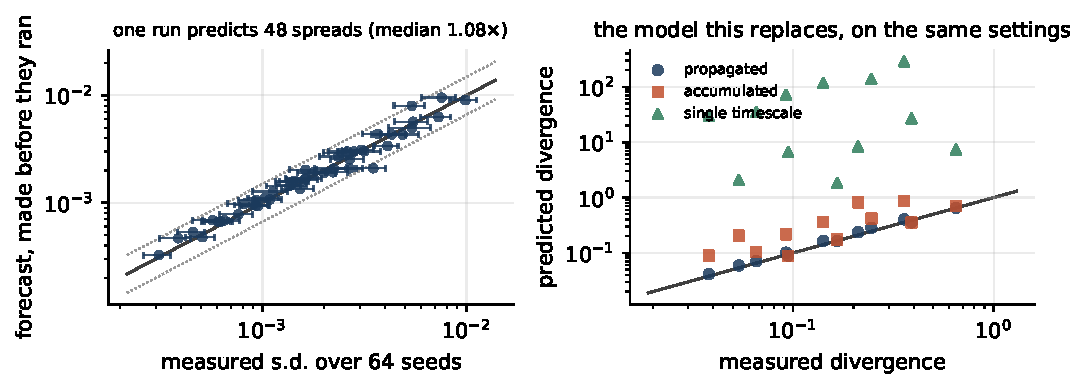
\includegraphics[width=\textwidth]{figures/teaser.pdf}}
    \captionof{figure}{\textbf{Left:} the efficiency $\rho(G)$ predicted from two measured traces
    with no fitted parameters, against the gain actually obtained by training at that split.
    Settings differ in run length and task, so both axes are standardised within a setting; what is
    pooled is the shape. \textbf{Right:} the optimal group size from Theorem~\ref{thm:split} at that
    measured noise ratio, against the rollout budget, for the prefill ratios $\alpha$ we measure on
    real hardware. Statistics alone say three; the hardware says the rest, and says something
    different for long prompts with short answers than for reasoning-length responses.}
    \label{fig:teaser}
  \end{minipage}
  \vspace{10pt}
]

\renewcommand{\thefootnote}{\textdagger}
\footnotetext{ETH Z\"urich neither endorsed nor funded this work. The author was a BSc Computer
Science student throughout this research, which is the source of the affiliation.}
\renewcommand{\thefootnote}{\arabic{footnote}}


\section{Introduction}
\label{sec:introduction}

A paper reports that reinforcement learning post-training moved a benchmark by two points. Whether
that is a result depends on a number nobody has: how much the same recipe would have moved it with
a different seed. The problem is documented \citep{henderson2018matters, hochlehnert2025sober} and
the only instrument the field has is replication, which at current RL compute is close to
unaffordable. So the number usually goes unmeasured.

Start from the obvious model. Gradient noise perturbs each update, perturbations accumulate, two
runs execute a random walk away from each other, and reproducibility decays with run length. That
picture is implicit in how run-to-run variance is discussed, and it is what a noisy gradient
suggests.

It is wrong, and the way it is wrong is the subject of this paper. Noise from one update does not
survive to the end of training unchanged. It is passed through every update that follows, and where
the shared objective is locally concave those updates shrink it. What reaches the end is a
convolution of injected noise with the sensitivity of the remaining trajectory, and that object is
computable.

\paragraph{Contributions.}
\begin{itemize}
  \item \textbf{A finite-time covariance law} (Theorem~\ref{thm:propagation}).
  $S_{t+1} = A_t S_t A_t^{\!\top} + Q_t$, giving expected divergence between seeds as
  $\tr(F_T S_T)$ and attributing it to individual updates through a per-update kernel. In an
  exactly solvable policy it predicts measured divergence to $9\%$ at the median over twelve
  settings, against $2.0\times$ for accumulation and two orders of magnitude for a single-timescale
  approximation.

  \item \textbf{The contraction is caused by learning.} Replacing rewards with coin flips, which
  leaves noise and batch composition untouched, turns a flat divergence trace into one that grows
  $10.7\times$ over eighty updates. This separates the result from a claim that seeds merely end up
  nearby.

  \item \textbf{The machinery that makes the injected noise measurable}: an exact finite-$G$ mean
  and covariance for the count-based advantage estimators under binary rewards
  (Propositions~\ref{prop:mean} and \ref{prop:cov}), a decomposition of the gradient noise into
  between-prompt and within-prompt terms, and an estimator that recovers both from the microbatch
  gradients a trainer already accumulates. The same decomposition fixes the compute-optimal group
  size (Theorem~\ref{thm:split}), which we validate prospectively.

  \item \textbf{An explicit account of what does not hold.} A single contraction timescale fails by
  two orders of magnitude, and we report it as the comparator rather than the law. A predicted
  square-root relation between policy divergence and outcome spread is not supported by our data
  and is withdrawn. Drift-targeted control, which Section~\ref{sec:drift} otherwise recommends,
  destroys runs at saturation. The largest model we measure is $0.5$B, which bounds what any of
  this establishes about frontier-scale RLVR.
\end{itemize}

Every experiment here runs on one laptop, which sets the ceiling on the last point and is stated
plainly in Section~\ref{sec:discussion} rather than left for a reader to infer.

\section{Setup}
\label{sec:setup}

A policy $\policy(y \mid x)$ generates a response $y$ to a prompt $x \sim \mathcal{D}$, and a
verifier returns a binary reward $r(x,y) \in \{0,1\}$. The objective is the expected pass rate
\begin{equation}
  J(\theta) \;=\; \E_{x \sim \mathcal{D}} \, \E_{y \sim \policy(\cdot \mid x)}\big[ r(x,y) \big]
  \;=\; \E_{x}\big[ p(x) \big], \qquad p(x) := \Pr\big[ r = 1 \mid x \big].
\end{equation}
Write $\score(y) := \nabla_\theta \log \policy(y \mid x)$ for the score, so that
$\E_{y}[\score] = 0$, and let $u_r := \E[\score \mid r]$ and $S_r := \Cov(\score \mid r)$ be the
mean and covariance of the score conditional on the reward. The zero-mean property of the score
gives the identity used throughout,
\begin{equation}
  \label{eq:score-identity}
  p\,u_1 + (1-p)\,u_0 = 0
  \qquad\Longrightarrow\qquad
  u_0 = -\tfrac{p}{1-p}\, u_1 ,
\end{equation}
and the per-prompt gradient is $h(x) := \E_y[r\,\score] = p\, u_1$. Because the reward is binary,
every quantity in this paper depends on the policy only through the four per-prompt objects
$(p, u_1, S_0, S_1)$. That reduction is what makes an exact finite-$G$ theory possible.

\paragraph{Batches.} A batch consists of $P$ prompts drawn independently from $\mathcal{D}$ and $G$
responses drawn independently from the policy for each prompt. We call $G$ the \emph{group size}
and $R = PG$ the \emph{rollouts per step}. Hardware fixes $R$; how to split it is the question.

\paragraph{The estimator family.} Let $k = \sum_{j} r_j$ be the number of successes in a group. We
consider any advantage of the form
\begin{equation}
  \label{eq:family}
  A_j \;=\; w(k, r_j),
\end{equation}
that is, any rule in which a response's advantage depends only on its own reward and on how many
of its group-mates succeeded. This covers the estimators in current use, each of which is fully
described by a $(G+1) \times 2$ table:

\begin{center}
\begin{tabular}{ll}
  \toprule
  estimator & $w(k, r)$ \\
  \midrule
  RLOO \citep{ahmadian2024rloo} & $r - (k - r)/(G-1)$ \\
  GRPO with a mean baseline \citep{liu2025drgrpo} & $r - k/G$ \\
  GRPO, standardised \citep{shao2024deepseekmath} & $\big(r - k/G\big) \big/ \sqrt{(k/G)(1 - k/G)}$, zero when $k \in \{0, G\}$ \\
  fixed external baseline & $r - \hat{p}$ \\
  \bottomrule
\end{tabular}
\end{center}

The per-prompt estimator and the batch estimator are
\begin{equation}
  z \;:=\; \frac{1}{G}\sum_{j=1}^{G} w(k, r_j)\, \score(y_j),
  \qquad
  \ghat \;:=\; \frac{1}{P}\sum_{i=1}^{P} z_i .
\end{equation}
Token-level reshaping of the advantage, length normalisation and clipping fall outside
\eqref{eq:family}; Section~\ref{sec:discussion} returns to them.

\section{What the estimators compute, and how noisy they are}
\label{sec:theory}

All results in this section are exact at finite $G$, and all are verified against brute-force
enumeration in Section~\ref{sec:experiments}. Define, for $m \sim \mathrm{Binomial}(G-1, p)$ and
$m' \sim \mathrm{Binomial}(G-2, p)$,
\begin{equation}
  \label{eq:contractions}
  W_r := \E_m\big[w(r + m, r)\big], \quad
  Q_r := \E_m\big[w(r + m, r)^2\big], \quad
  C_{ab} := \E_{m'}\big[w(a + b + m', a)\, w(a + b + m', b)\big].
\end{equation}

\subsection{The estimator zoo is a reweighting of prompt difficulty}

\begin{proposition}[Exact expectation]
  \label{prop:mean}
  For any estimator of the form \eqref{eq:family} and any binary reward,
  \begin{equation}
    \E[z \mid x] \;=\; \lambda(p, G)\, h(x),
    \qquad
    \lambda(p, G) \;=\; W_1(p,G) - W_0(p,G).
  \end{equation}
\end{proposition}

\begin{proof}
  Condition on $r_j$. The other $G-1$ rewards are i.i.d.\ Bernoulli$(p)$ and, given $r_j$, are
  independent of $\score(y_j)$, so
  $\E[w(k, r_j)\score(y_j)] = \sum_{r} \Pr[r]\, W_r\, u_r$. Summing over $j$ and applying
  \eqref{eq:score-identity} gives $\E[z] = p\,(W_1 - W_0)\,u_1 = \lambda h$.
\end{proof}

Three consequences follow immediately, and each is exact for every $p$ and every $G$.
RLOO has $W_1 = 1-p$ and $W_0 = -p$, hence $\lambda \equiv 1$: it is unbiased.
GRPO with a mean baseline has $\lambda = (G-1)/G$, independent of $p$: it is RLOO multiplied by a
constant. Standardised GRPO has a $\lambda(p, G)$ with no closed form but an exact binomial sum.

So no member of this family points in the wrong direction. Each computes the true per-prompt
gradient $h(x)$, scaled by a weight that depends on the prompt's difficulty; the family optimises
the reweighted gradient field $\E_x[\lambda(p(x), G)\, h(x)]$, and its members differ only through
$\lambda$. Standardisation is therefore not a variance-reduction device. It is a change of
objective, one that upweights prompts whose pass rate is near $0$ or $1$ relative to prompts of
intermediate difficulty.

A constant $\lambda$ is invisible: rescaling an estimator by $c$ rescales the optimal step size by
$1/c$ and leaves every trajectory unchanged. Only the \emph{dependence of $\lambda$ on $p$} can
alter what a run converges to. This is the sense in which most of the zoo is one estimator.

\subsection{Exact covariance at finite group size}

\begin{proposition}[Exact per-prompt covariance]
  \label{prop:cov}
  With $U := u_1 u_1^{\!\top}$,
  \begin{equation}
    \Cov(z \mid x)
    = \frac{1}{G}\Big[ p\,Q_1 S_1 + (1-p)\,Q_0 S_0 \Big]
    + c_U(p, G)\, U ,
  \end{equation}
  \begin{equation}
    c_U = \frac{1}{G}\Big( p\,Q_1 + \frac{p^2 Q_0}{1-p} \Big)
        + p^2\Big[ \frac{G-1}{G}\big( C_{11} - 2C_{10} + C_{00} \big) - \lambda^2 \Big].
  \end{equation}
\end{proposition}

\begin{proof}
  Split $\E[z z^{\!\top}]$ into diagonal and off-diagonal terms. The diagonal contributes
  $G^{-1}[p Q_1 M_1 + (1-p) Q_0 M_0]$ with $M_r = S_r + u_r u_r^{\!\top}$. For $j \neq l$,
  condition on $(r_j, r_l)$ and on the count $m'$ among the remaining $G-2$ responses; the two
  scores are then conditionally independent, giving
  $\frac{G-1}{G}\sum_{a,b}\Pr[a]\Pr[b]\,C_{ab}\,u_a u_b^{\!\top}$, which collapses to
  $\frac{G-1}{G} p^2 (C_{11} - 2C_{10} + C_{00}) U$ by \eqref{eq:score-identity}. Subtracting
  $\E[z]\E[z]^{\!\top} = \lambda^2 p^2 U$ completes the proof.
\end{proof}

\subsection{Two levels of noise}

Prompts are drawn independently, so with $\gbar := \E_x[\lambda h]$ the batch estimator has
\begin{equation}
  \label{eq:hierarchy}
  \Cov(\ghat) \;=\; \frac{1}{P}\Big[ \Sb + \Sw \Big],
  \qquad
  \Sb := \Cov_x\big( \lambda(p(x), G)\, h(x) \big),
  \qquad
  \Sw := \E_x\big[ \Cov(z \mid x) \big].
\end{equation}
$\Sb$ is the irreducible variance of sampling prompts and does not shrink with $G$; $\Sw$ is the
variance of sampling responses and does. Pretraining has one level of sampling and therefore one
noise scale. RLVR has two, and the split of a fixed rollout budget between them is a free choice
that nothing in the literature currently determines.

\begin{corollary}[The reward histogram predicts the response-level noise]
  \label{cor:bernoulli}
  For RLOO, $p Q_1 + (1-p) Q_0 = p(1-p)\,G/(G-1)$ exactly, for every $G$. If the conditional score
  covariances are comparable across the two reward classes, $\tr S_0 \approx \tr S_1 \approx
  \sigma_s^2$, then
  \begin{equation}
    \label{eq:bernoulli}
    \tr \Sw \;\approx\; \frac{\sigma_s^2}{G-1}\, \E_x\big[ p(x)\,(1 - p(x)) \big].
  \end{equation}
\end{corollary}

The response-level noise is, up to one slowly varying scalar, the mean Bernoulli variance of the
pass-rate distribution: a quantity every RLVR trainer already logs, at no cost. The isotropy
assumption is measured rather than asserted in Section~\ref{sec:experiments}.

\section{Drift, efficiency, and how to split a rollout budget}
\label{sec:drift}

The usual route to a critical batch size is a second-order model of the objective
\citep{mccandlish2018empirical}. It does not survive contact with RLVR. The objective $J = \E[r]$
is not a log-likelihood, its Hessian is not the negative Fisher information, and along a policy
gradient direction a log-linear policy keeps improving well past the step at which a quadratic
model turns over. Measured against exactly computed improvement in
Section~\ref{sec:experiments}, the curvature model understates the useful step size by more than a
factor of four.

What is accurate is a model of how far the policy moves.

\subsection{The drift model}

One update of size $\eta$ displaces the policy by
\begin{equation}
  \label{eq:drift}
  D(\eta) \;:=\; \E_x\Big[ \KL\big( \pi_{t+1}(\cdot \mid x) \,\big\|\, \pi_t(\cdot \mid x) \big) \Big]
  \;=\; \tfrac{1}{2}\eta^2\, \E\big[ \ghat^{\!\top} F\, \ghat \big] + O(\eta^3)
  \;=\; \tfrac{1}{2}\eta^2 \Big( \mathcal{G} + \tfrac{N}{P} \Big),
\end{equation}
where $F$ is the Fisher information of the policy,
$\mathcal{G} := \gbar^{\!\top} F \gbar$ and $N := \tr(F\Sb) + \tr(F\Sw)$. In the enumerable
testbed \eqref{eq:drift} predicts the true KL to within $3\%$ over three orders of magnitude in
$\eta$.

Drift decomposes into a \emph{signal} part $\tfrac{1}{2}\eta^2\mathcal{G}$, which moves the policy
along the mean update, and a \emph{diffusive} part $\tfrac{1}{2}\eta^2 N/P$, which is a random walk
in function space and buys nothing. Their ratio defines the efficiency
\begin{equation}
  \label{eq:efficiency}
  \rho \;:=\; \frac{\mathcal{G}}{\mathcal{G} + N/P} \;=\; \frac{1}{1 + \Bcrit/P},
  \qquad
  \Bcrit \;:=\; \frac{N}{\mathcal{G}} \;=\; \frac{\tr(F\Sb) + \tr(F\Sw)}{\gbar^{\!\top} F \gbar},
\end{equation}
which is the RLVR analogue of the gradient noise scale, measured in prompts, and is a two-level
quantity: a floor set by prompt diversity plus a term that $G$ divides down. Equation
\eqref{eq:efficiency} also says that \textbf{a trainer can read its own batch-size efficiency off
the KL it already logs}: a run whose measured drift is mostly diffusive is running below its
critical batch size, and by how much is quantified without a sweep.

\subsection{Progress at a fixed drift budget}

To first order an update improves the objective by $\eta\, a$ with $a := \nabla J^{\!\top}\gbar$.
Solving \eqref{eq:drift} for $\eta$ at a prescribed drift $D$,
\begin{equation}
  \label{eq:progress}
  \E[\Delta J] \;=\; a\sqrt{\frac{2D}{\mathcal{G} + N/P}}
  \;=\; \sqrt{2D}\;\frac{a}{\sqrt{\mathcal{G}}}\;\sqrt{\rho}.
\end{equation}
Progress at a fixed drift budget scales as the \emph{square root} of the efficiency. The estimator
enters only through $a/\sqrt{\mathcal{G}}$, the alignment of its mean with the true gradient in
Fisher units; the batch composition enters only through $\rho$.

Since KL is quadratic in the step, a fixed total drift $D_{\mathrm{tot}}$ spread over $N_{\text{s}}$
updates buys path length $\propto \sqrt{N_{\text{s}} D_{\mathrm{tot}}}$: many small steps travel
further than one large step of the same total drift. Total progress over a run therefore scales as
$\sqrt{N_{\text{s}}\,\rho}$, and maximising it over the batch composition means maximising
$N_{\text{s}}\rho$.

\subsection{The optimal group size}

Let $\tau_b := \tr(F\Sb)$ and $\tau_w := (G-1)\tr(F\Sw)$, the latter independent of $G$ to leading
order by Corollary~\ref{cor:bernoulli}. With the rollouts per step $R = PG$ fixed by hardware,
maximising $N_{\text{s}}\rho = R_{\mathrm{tot}} / \big( G (P + \Bcrit(G)) \big)$ means minimising
\begin{equation}
  \label{eq:objective}
  G\,\Bcrit(G) \;=\; \frac{1}{\mathcal{G}}\Big[ G\,\tau_b + \tau_w\,\frac{G}{G-1} \Big],
\end{equation}
which is convex in $G$ with an interior minimum.

\begin{proposition}[Optimal group size]
  \label{prop:gstar}
  At a fixed number of rollouts per step,
  \begin{equation}
    \label{eq:gstar}
    G^{*} \;=\; 1 + \sqrt{\frac{\tau_w}{\tau_b}} ,
  \end{equation}
  independently of $R$. Holding $P$ fixed instead gives
  $G^{*} = 1 + \sqrt{\tau_w / (P\mathcal{G} + \tau_b)}$, which recovers \eqref{eq:gstar} when the
  run is below its critical batch size.
\end{proposition}

The optimal group size is one plus the square root of the ratio of within-prompt to
between-prompt gradient noise. Both traces are measurable from a single batch
(Section~\ref{sec:estimation}), so $G^{*}$ is an observable rather than a hyperparameter.

\paragraph{Rollouts are not equally expensive.} When a group shares its prompt's prefix, prefill is
paid once per prompt and decode once per response, so the cost of a step is
$P\,(c_{\mathrm{pre}} + G\,c_{\mathrm{dec}})$. Minimising
$(c_{\mathrm{pre}} + G c_{\mathrm{dec}})\Bcrit(G)$ in place of \eqref{eq:objective} gives
\begin{equation}
  \label{eq:gstar-cost}
  G^{*}_{\mathrm{compute}} \;=\; 1 + \sqrt{\Big(1 + \frac{c_{\mathrm{pre}}}{c_{\mathrm{dec}}}\Big)
  \frac{\tau_w}{\tau_b}} .
\end{equation}
The compute-optimal group size is the statistically optimal one inflated by
$\sqrt{1 + c_{\mathrm{pre}}/c_{\mathrm{dec}}}$. Two measurements fix it: the noise ratio from the
trainer and the prefill-to-decode cost ratio from the serving stack.

\paragraph{The optimum moves during a run.} Both $\tau_w$ and $\tau_b$ change as the policy
improves: $\E_x[p(1-p)]$ falls once a task is largely solved, and prompt-to-prompt gradient
heterogeneity falls as a model acquires a shared algorithm. Which effect dominates is an empirical
question, not a theoretical one, and Section~\ref{sec:experiments} shows both directions occurring
in different settings. This is the point of the paper in miniature: the schedule is measurable, and
it is not guessable.

\subsection{The step size is a drift target}

Equation \eqref{eq:drift} inverts to
$\eta(D) = \sqrt{2D / (\mathcal{G} + N/P)}$, so a run can be specified by a target drift instead of
a learning rate. Learning rate, clip range and KL coefficient are three controls acting on the
single quantity $D$, which is why they interact, and why none of them transfers between scales or
tasks on its own. Drift is measured in nats per token and is a property of the policy's behaviour
rather than of its parameterisation; whether that makes it transfer is tested in
Section~\ref{sec:experiments}.

\section{From one run to the spread of its result}
\label{sec:seeds}

Fix a policy $\theta_0$ and start two runs from it. They see the same prompts and the same
objective, and differ only in the randomness of their rollouts. This is the comparison a
practitioner makes when they change a seed and rerun, and the question this section answers is how
far apart the numbers they report end up --- using only one of the runs.

\subsection{Noise is filtered, not accumulated}

Write $\Delta_t := \theta^A_t - \theta^B_t$. With updates $\theta \leftarrow \theta + \eta\ghat$
and $J_t := \partial\gbar/\partial\theta$ the Jacobian of the mean update,
\begin{equation}
  \label{eq:seed-recursion}
  \Delta_{t+1} = A_t \Delta_t + \eta\,\nu_t,
  \qquad A_t := I + \eta J_t,
\end{equation}
to first order in $\Delta$, with $\Cov(\nu_t) = 2\Sigma_t/P$. The batch noise $\Sigma_t$ is left abstract here and made
explicit in Section~\ref{sec:theory}, where it is computed exactly at finite group size; nothing
in this section depends on which estimator produced it.

If the objective were flat, $J = 0$, this would be a random walk: divergence would accumulate,
$\E\|\Delta_t\|^2 \propto t$, and a longer run would be strictly less reproducible than a short one.
That is the implicit model behind treating run-to-run variance as something to be measured by
brute force. But two RLVR runs are climbing the same objective, and where it is locally concave
$A_t$ is a contraction: divergence injected at one update decays over the ones that follow.

The consequence is that noise from update $t$ is not added to the final divergence. It is passed
through every subsequent update first.

\begin{theorem}[Finite-time covariance]
  \label{thm:propagation}
  Let $S_t$ denote the covariance of a run about its mean trajectory, with $S_0 = 0$ when both runs
  start from the same policy. Under the linearisation \eqref{eq:seed-recursion},
  \begin{equation}
    \label{eq:lyapunov}
    S_{t+1} = A_t S_t A_t^{\!\top} + Q_t,
    \qquad Q_t := \eta^2 \Sigma_t / P,
  \end{equation}
  and therefore
  \begin{equation}
    \label{eq:unrolled}
    S_T = \sum_{t=0}^{T-1} \Phi_{T,t+1}\, Q_t\, \Phi_{T,t+1}^{\!\top},
    \qquad \Phi_{T,s} := \!\!\prod_{u=s}^{T-1}\!\! A_u ,
  \end{equation}
  the product taken in order of decreasing $u$.
  Two independent seeds satisfy $\Cov(\theta^A_T - \theta^B_T) = 2S_T$, so their expected policy
  divergence is
  \begin{equation}
    \label{eq:predicted-kl}
    \E\big[\KL(\pi^A \,\|\, \pi^B)\big] \;\approx\; \tr\!\big(F_T\, S_T\big).
  \end{equation}
\end{theorem}

\begin{proof}
  Taking the covariance of \eqref{eq:seed-recursion} for a single run about its mean and using
  independence of $\nu_t$ from $\Delta_t$ gives \eqref{eq:lyapunov}; unrolling it from $S_0 = 0$
  gives \eqref{eq:unrolled}. Two independent runs have independent noise, so the covariance of
  their difference is twice that of one about the mean. Expanding
  $\KL(\pi^A\|\pi^B) \approx \tfrac{1}{2}\Delta^{\!\top}F\Delta$ and taking expectations gives
  $\tfrac{1}{2}\tr(F\cdot 2S_T)$.
\end{proof}

Equation \eqref{eq:unrolled} is the object this section is about, and it is worth reading as a
convolution: what survives to the end is the noise injected at each update, weighted by how
strongly the remaining trajectory preserves a perturbation entering there. Write
\begin{equation}
  \label{eq:kernel}
  k_t \;:=\; \tr\!\big(F_T\, \Phi_{T,t+1} Q_t \Phi_{T,t+1}^{\!\top}\big),
  \qquad
  \E[\KL] = \sum_{t} k_t,
\end{equation}
for the contribution of update $t$. Two runs are not equally sensitive to noise at every point in
training, and $k_t$ says where the sensitivity is.

\subsection{Why a single timescale is not enough}

An earlier version of this work replaced the spectrum of $A_t$ by one effective eigenvalue,
giving $\E[\KL_\infty] = \tau_c D_{\mathrm{noise}}$ for a persistence time $\tau_c$. That
approximation is the natural first move and it fails badly:
Section~\ref{sec:exp-seeds} measures it at a median error of two orders of magnitude, against
$9\%$ for \eqref{eq:unrolled}. The reason is visible in \eqref{eq:unrolled}. $A_t$ has a spectrum,
fast directions equilibrate within a few updates while slow ones set the final level, and a single
fitted exponential is pinned by the early rise and blind to what dominates the answer. We report
the scalar law only as the comparator it turned out to be.

\subsection{What the recursion predicts}

\paragraph{Divergence stops growing when, and because, the run is learning.} Contraction requires
$J_t$ to be meaningfully negative definite, which requires a signal. With no learning signal
\eqref{eq:seed-recursion} degenerates to a random walk. This is testable directly by removing the
signal while leaving the noise untouched, which Section~\ref{sec:exp-seeds} does.

\paragraph{The level is set by batch composition.} $Q_t \propto \Sigma_t/P$, so halving the
injected noise requires quadrupling the batch, and nothing in \eqref{eq:unrolled} depends on the
number of updates once the sum has converged.

\paragraph{A memory horizon, if contraction is strong enough to make one.} If $\Phi_{T,t+1}$
decays with $T - t$, the sum in \eqref{eq:unrolled} is dominated by its last terms and the final
$h \ll T$ updates account for nearly all of the spread; reproducing a result would then mean
reproducing its end. Where contraction is weak, $k_t$ is flat and every update counts the same.
Section~\ref{sec:exp-seeds} asks which of these holds and finds the second, over every setting we
can reach.

\subsection{Carrying it to the number that gets reported}
\label{sec:metric}

Equation \eqref{eq:predicted-kl} is a statement about policies. What a paper reports is a score:
pass rate, exact match, win rate, mean reward. Write $M(\theta)$ for that score as a function of
the parameters. Linearising it about the endpoint the run reached,
\begin{equation}
  \label{eq:metric-variance}
  \Var_{\text{seed}}\big[M(\theta_T)\big] \;\approx\; \nabla M(\theta_T)^{\!\top} S_T\, \nabla M(\theta_T),
\end{equation}
which needs $S_T$ --- a matrix nobody can form for a real model. It is not needed. Substituting
\eqref{eq:unrolled} turns the quadratic form into a sum of scalars.

\begin{theorem}[Adjoint form of the reported spread]
  \label{thm:adjoint}
  Define $b_T := \nabla M(\theta_T)$ and $b_s := A_s^{\!\top} b_{s+1}$ for $s = T-1, \dots, 0$.
  Then, under the assumptions of Theorem~\ref{thm:propagation},
  \begin{equation}
    \label{eq:adjoint}
    \begin{aligned}
      \Var_{\text{seed}}\big[M(\theta_T)\big]
      &\;=\; \sum_{t=0}^{T-1} b_{t+1}^{\!\top} Q_t\, b_{t+1} \\
      &\;=\; \frac{\eta^2}{P}\sum_{t=0}^{T-1} \Var\!\big(b_{t+1}^{\!\top}\hat{g}_t\big),
    \end{aligned}
  \end{equation}
  where the variance on the right is over one batch at $\theta_t$.
\end{theorem}

\begin{proof}
  $b_s = \Phi_{T,s}^{\!\top}\nabla M$ by induction. Substituting \eqref{eq:unrolled} into
  \eqref{eq:metric-variance} gives $\sum_t (\Phi_{T,t+1}^{\!\top}\nabla M)^{\!\top} Q_t
  (\Phi_{T,t+1}^{\!\top}\nabla M)$. The second equality is $Q_t = \eta^2\Sigma_t/P$ and
  $b^{\!\top}\Sigma b = \Var(b^{\!\top}\hat{g})$.
\end{proof}

Every term of \eqref{eq:adjoint} is the variance of a batch gradient projected onto a single
direction --- one scalar per update, which a trainer can accumulate alongside the update it is
already making. What the backward pass costs depends on $A_s^{\!\top}$, and here the estimator
family pays for itself.

\begin{proposition}[The mean update is a gradient field]
  \label{prop:potential}
  For any count-based estimator, $\gbar(\theta) = \nabla_\theta\,\Phi(\theta)$ with
  $\Phi(\theta) = \E_x[\Lambda(p_x)]$ and $\Lambda' = \lambda$. Hence $J = \nabla^2\Phi$ is
  symmetric and $A_s^{\!\top} = A_s$.
\end{proposition}

\begin{proof}
  By Proposition~\ref{prop:mean}, proved in Section~\ref{sec:theory}, the per-prompt mean is
  $\lambda(p_x, G)\,\nabla_\theta p_x$, and
  $\lambda$ depends on $\theta$ only through $p_x$. So
  $\lambda(p_x)\nabla p_x = \nabla \Lambda(p_x)$, and averaging over $x$ commutes with the
  gradient.
\end{proof}

The backward pass is therefore a Hessian-vector product, which finite differences deliver from two
gradient evaluations and reverse mode from one double backward. Neither $J$ nor $S_T$ is ever
formed. For RLOO, where $\lambda \equiv 1$, the potential is the pass rate itself: the mean update
ascends exactly the quantity being reported.

Two consequences worth stating plainly. First, this is a \emph{forecast}: \eqref{eq:adjoint} reads
only the states one run visited, so it can be computed before any second run exists, which is how
Section~\ref{sec:exp-seeds} tests it. Second, restricting $\Sigma_t$ to one of its two terms
attributes the answer by origin --- $\Sigma_b$ is which prompts were drawn, $\Sigma_w$ is which
responses were sampled --- and the two shares are exact and sum to one.

\subsection{Where the argument stops}

Everything above linearises the update around the shared trajectory, which requires the two runs to
stay close enough for $\gbar$ to be locally linear between them, and requires
$\eta\|J_t\| \ll 1$. Both fail when the step grows relative to the curvature, and RLVR supplies a
concrete way for that to happen: a controller holding drift at a fixed target must raise $\eta$ as
the signal decays, and $\E_x[p(1-p)] \to 0$ as a task is solved takes the signal with it.
Section~\ref{sec:exp-seeds} shows runs crossing out of the regime exactly this way.

\section{Measuring the two noise scales from a single batch}
\label{sec:estimation}

Both $\tau_b$ and $\tau_w$ are recoverable from gradients a trainer already computes. Partition the
batch by prompt half and by rollout sub-group, and accumulate the four resulting microbatch
gradients separately:
\begin{equation}
  g_{ab} \;:=\; \text{mean gradient over prompt half } a \text{ using rollout sub-group } b,
  \qquad a, b \in \{0, 1\},
\end{equation}
each computed with its own sub-group's advantages. The two prompt halves are independent, and
given a prompt the two sub-groups are independent, so every term below is an inner product of
independent quantities:
\begin{align}
  \label{eq:estimators}
  \gbar^{\!\top} M \gbar &= \E\big[ g_{00}^{\!\top} M\, g_{11} \big],
  &&\text{different prompts, different responses,} \\
  \tr(M\Sb) &= \tfrac{P}{2}\Big( \E\big[ g_{a0}^{\!\top} M\, g_{a1} \big]
                                 - \E\big[ g_{00}^{\!\top} M\, g_{11} \big] \Big),
  &&\text{same prompts, different responses,} \nonumber \\
  \tr(M\Sw) &= \tfrac{P}{4}\, \E\big[ \| g_{a0} - g_{a1} \|_M^2 \big],
  &&\text{the prompt term cancels in the difference.} \nonumber
\end{align}

The cost is four gradient buffers rather than one, no extra responses, and no extra backward work
beyond accumulating into four accumulators instead of one -- which any trainer using gradient
accumulation over microbatches is already doing. Setting $M = I$ gives the practical form; setting
$M = F$ is obtained from measured KL rather than from materialising the Fisher.

\paragraph{Conditioning.} The obvious alternative, estimating the total variance and subtracting
the within-prompt part, is a difference of two large and highly correlated variances. On
homogeneous prompt pools it routinely returns a negative $\tau_b$ and an infinite $G^{*}$. The form
in \eqref{eq:estimators} differences two quantities of comparable size that share no sampling
noise, and it tracked the exact $\tau_b$ to within $4\%$ across pools spanning a factor of seven in
$G^{*}$ where the subtractive form failed outright.

\paragraph{Preconditioners.} An update is $\eta\, \Pi\, \ghat$ for a preconditioner $\Pi$, and Adam
is scale invariant, so both the drift model and the estimators must be read in the metric the
update actually moves in. In practice this means instrumenting the preconditioned gradient: all
results in \eqref{eq:estimators} carry over with $F \mapsto \Pi F \Pi$ under the standard
assumption that $\Pi$ varies slowly relative to batch-to-batch fluctuation.

\paragraph{Controlling drift.} Since $D \propto \eta^2$, a multiplicative controller
\begin{equation}
  \eta_{t+1} \;=\; \eta_t \cdot \mathrm{clip}\Big( \big( D^{*} / D_t \big)^{1/2},\ c^{-1},\ c \Big)
\end{equation}
corrects a mis-set step in a single update when the drift estimate is clean. Measured over runs on
transformers, this controller holds the median drift at its target with no detectable bias in log
space. Exponential smoothing of $D_t$, the obvious refinement, makes it worse: the lag biases the
realised drift low by roughly a factor of two.

\section{Experiments}
\label{sec:experiments}

Three levels of evidence. Policies small enough to enumerate, where the objective, the Fisher
information, the drift and both noise terms are computed rather than estimated. Transformers trained
from scratch, where a population of independent runs executes as one batched kernel so that sweeps
carry standard errors rather than anecdotes. And a pretrained model, where the same measurement is
made on a real policy and a real verifier. Everything ran on a single Apple M4 laptop.

\subsection{How training noise reaches the end of a run}
\label{sec:exp-seeds}

\paragraph{The recursion predicts divergence; a single timescale does not.} The enumerable policy
admits three things at once: the exact linearised recursion \eqref{eq:lyapunov}, the exact Fisher
information, and as many independent stochastic trajectories as we care to run. That allows
candidate models of seed divergence to be scored against ground truth rather than against each
other. Over twelve settings spanning prompt diversity, group size, batch size and step size, we
compare the propagated covariance against two alternatives: accumulation with no contraction, and
the single-timescale law an earlier version of this work relied on.

\begin{table}[t]
  \centering
  \small
  \begin{tabular}{lccc}
\toprule
model of seed divergence & median error & worst & range of ratio \\
\midrule
propagated covariance, \eqref{eq:unrolled} & 1.09$\times$ & 1.2$\times$ & 0.92--1.17 \\
accumulation, no contraction & 2.00$\times$ & 3.9$\times$ & 0.91--3.89 \\
single timescale & 194.84$\times$ & 844.0$\times$ & 11.17--843.99 \\
\bottomrule
\end{tabular}
  \caption{Predicted against measured divergence between independent runs in the enumerable policy,
  with $300$ trajectories per setting. Error is the ratio of predicted to measured, summarised as
  $\exp$ of the median absolute log ratio.}
  \label{tab:propagation}
\end{table}

The propagated recursion is accurate to $9\%$ at the median and $17\%$ at worst. Ignoring
contraction overshoots by up to $3.9\times$, and does so exactly where the policy is learning:
on the most homogeneous prompt pools, where the objective supplies the most curvature, it is wrong
by a factor of two and a half, while on heterogeneous pools where little learning happens it is
indistinguishable from the truth. The single-timescale law is wrong by two orders of magnitude.
That failure is informative rather than embarrassing: it is what \eqref{eq:unrolled} predicts when
a spectrum of contraction rates is compressed to one number.

\paragraph{Contraction requires a learning signal.} If divergence stops growing because the shared
objective pulls two runs together, then removing the objective while leaving the noise in place
should restore accumulation. We ran a population of transformers twice from identical parameters:
once normally, and once with every reward replaced by an independent coin flip, which leaves the
rollout sampling, the batch composition and the gradient magnitudes intact while destroying the
learning signal.

\begin{table}[t]
  \centering
  \small
  \begin{tabular}{lcccc}
    \toprule
    & \multicolumn{2}{c}{learning} & \multicolumn{2}{c}{signal removed} \\
    \cmidrule(lr){2-3}\cmidrule(lr){4-5}
    updates & divergence & pass rate & divergence & pass rate \\
    \midrule
    1  & $1.15\times10^{-3}$ & 0.191 & $3.99\times10^{-3}$ & 0.184 \\
    20 & $1.26\times10^{-3}$ & 0.267 & $1.11\times10^{-2}$ & 0.177 \\
    40 & $1.35\times10^{-3}$ & 0.341 & $1.71\times10^{-2}$ & 0.185 \\
    80 & $0.94\times10^{-3}$ & 0.513 & $4.28\times10^{-2}$ & 0.184 \\
    \bottomrule
  \end{tabular}
  \caption{Divergence between runs that differ only in rollout randomness, with and without a
  learning signal. Same noise, same batches, same step sizes; only the rewards differ.}
  \label{tab:signal}
\end{table}

With a signal, divergence is flat while the pass rate climbs from $0.19$ to $0.51$. Without one it
grows by a factor of $10.7$ over the same eighty updates. The contraction is caused by the
objective, which is what \eqref{eq:seed-recursion} says and what separates this from a claim that
seeds happen to end up nearby.

\paragraph{On a pretrained model.} The transformers above are small and their task is synthetic.
We repeated the measurement on Qwen2.5-0.5B-Instruct with LoRA adapters, six runs differing only in
rollout randomness on exactly verifiable short-answer problems; because LoRA adapters start at zero
the runs begin from an identical policy by construction, and every checkpoint is scored on one fixed
batch of sequences.

\begin{figure}[t]
  \centering
  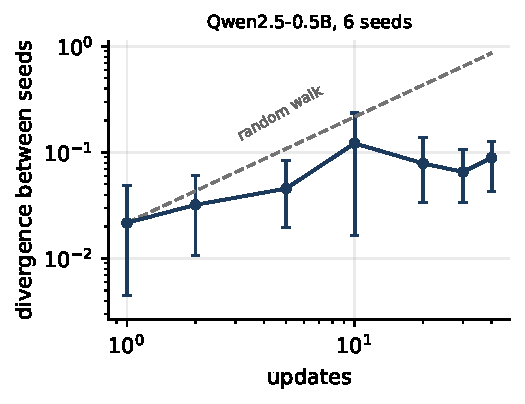
\includegraphics[width=0.9\linewidth]{figures/real_seeds.pdf}
  \caption{Divergence between six runs of a pretrained model differing only in rollout randomness.
  Intervals are $95\%$ bootstrap intervals resampled over runs rather than over pairs, since the
  fifteen pairwise distances are built from six runs. They are wide enough that the shape of the
  trace is not resolved; what is resolved is that the trace is not the dashed line.}
  \label{fig:real-seeds}
\end{figure}

Divergence reaches $1.22\times10^{-1}$ at ten updates and is $8.9\times10^{-2}$ at forty, with a
tail slope of $+0.14$ against the $+1$ accumulation requires. Two caveats belong with that number.
The fifteen pairwise distances come from six runs and are not independent, so intervals are
resampled over runs; doing so roughly doubles the standard error against treating the pairs as
independent. And once that is done the intervals at ten and forty updates overlap heavily, so the
apparent peak-and-fall is not resolved at six seeds. What the experiment supports is the weaker
statement that divergence does not accumulate on a pretrained model either. The six runs finish
within $0.835 \pm 0.044$ of each other in pass rate.

\paragraph{Bounded, not proven stationary.} Across the settings in which a run is still learning,
the log-log slope of divergence against update count runs from $-1.15$ to $+0.26$, against the
$+1$ that accumulation requires. That rejects accumulation. It does not establish stationarity in
the strict sense: $J_t$, $\Sigma_t$ and $\eta_t$ all move during training, so the level that
\eqref{eq:unrolled} converges to is itself slowly varying, and we describe the divergence as
bounded rather than stationary throughout.

\paragraph{How the level scales.} Compared at matched pass rate rather than matched step count,
a log-log fit over nine settings gives an exponent of $-0.61$ in the batch, $95\%$ CI
$[-1.42, +0.24]$, and $+0.59$ in the drift target, $95\%$ CI $[+0.27, +1.04]$, with $R^2 = 0.70$.
Both intervals contain the values $-1/2$ and $+1/2$ that follow from
$Q_t \propto \eta^2\Sigma/P$, and the batch interval also contains zero. Nine settings are too few
to pin a two-dimensional scaling law, and we report the intervals rather than the point estimates
for that reason.

\paragraph{What we do not claim.} An earlier version of this work predicted that the spread in
final task performance would follow $\sqrt{\KL_\infty}$. It does not, in our data: the fitted
exponent is $+0.10$ with $95\%$ CI $[-0.03, +0.45]$ against a predicted $+0.5$, and the interval
contains zero. Policy divergence and outcome spread are positively associated across our settings,
but these experiments do not establish the predicted relation, and we withdraw it. Predicting a
task metric directly, rather than through policy divergence, is the obvious route and we have not
taken it.

\subsection{Exactly enumerable policies}

The policy is a tabular autoregressive model over a small vocabulary, so its distribution over
sequences, its score at every sequence, and the conditional moments $(p, u_1, S_0, S_1)$ are
available exactly. Propositions~\ref{prop:mean} and~\ref{prop:cov} were checked against
brute-force enumeration over all $|\mathcal{Y}|^{G}$ group outcomes for five estimators and
$G \in \{2,3,4\}$: agreement to $10^{-12}$. The scaled within-prompt term $(G-1)\tr\Sw$, which the
theory treats as $G$-independent, varies by $6\%$ over $G = 2$ to $32$.

\paragraph{The curvature model fails, the drift model does not.} Taking a real update and computing
the resulting improvement and KL exactly, the second-order model of the objective places its optimal
step at least four times below the step that actually maximises improvement, which is where the
sweep ended, because $J = \E[r]$ is
not a log-likelihood and a log-linear policy keeps improving past the turnover of a quadratic model.
The drift model \eqref{eq:drift} predicts the measured KL to between $2.6\%$ and $3.9\%$ across a thousandfold range of step sizes. The theory in Section~\ref{sec:drift} is built on the second of these, not
the first.

\paragraph{Splitting a rollout budget.} For each prompt pool the parameter-free efficiency curve
$\rho(G)$ is compared against the improvement obtained by training at every split of a fixed budget,
holding total rollouts, total drift and step count fixed. Table~\ref{tab:exact-agreement} groups
pools by how much $\rho$ varies across the splits on offer.

\begin{table*}[t]
  \centering
  \begin{tabular}{lccc}
\toprule
predicted spread $\max\rho/\min\rho$ & pools & median $R^2$ & median Spearman \\
\midrule
$1.00$--$1.15$ & 8 & 0.670 & +0.588 \\
$1.15$--$1.35$ & 11 & 0.876 & +0.833 \\
$1.35$--$2.00$ & 6 & 0.971 & +0.957 \\
$2.00$--$8.00$ & 7 & 0.983 & +0.978 \\
\bottomrule
\end{tabular}
  \caption{Agreement between the predicted efficiency and the measured gain in the enumerable
  testbed, as a function of how strongly the prediction discriminates between splits. The prediction
  has no free parameters. Pools where it predicts that the split hardly matters are the pools where
  the measured curves are flat to within their standard errors.}
  \label{tab:exact-agreement}
\end{table*}

\begin{figure*}[t]
  \centering
  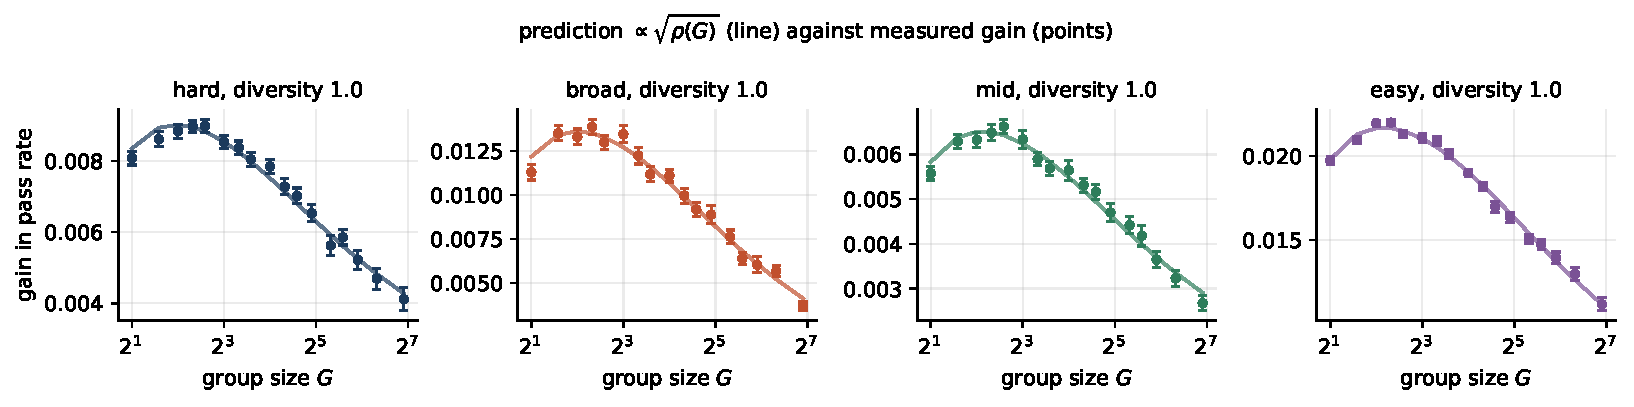
\includegraphics[width=0.95\textwidth]{figures/exact_curves.pdf}
  \caption{Measured gain against $\sqrt{\rho(G)}$ for the four pools whose predictions discriminate
  most strongly. Error bars are standard errors over seeds.}
  \label{fig:exact-curves}
\end{figure*}

\subsection{The estimator}

Figure~\ref{fig:estimator-accuracy} compares the group size recovered by the estimator of
Section~\ref{sec:estimation} against the exactly known value, over pools whose noise ratio spans a
factor of $26$ and whose $G^{\star}$ runs from $3.8$ to $15.2$. The median error in $G^{\star}$ is $1.3\%$
and the worst is $6.2\%$, using $2500$ batches of $32$ prompts split into $K = 8$ blocks; the
individual traces are recovered to $2.1\%$ ($\tau_w$) and $3.4\%$ ($\tau_b$) at the median.

\begin{figure}[t]
  \centering
  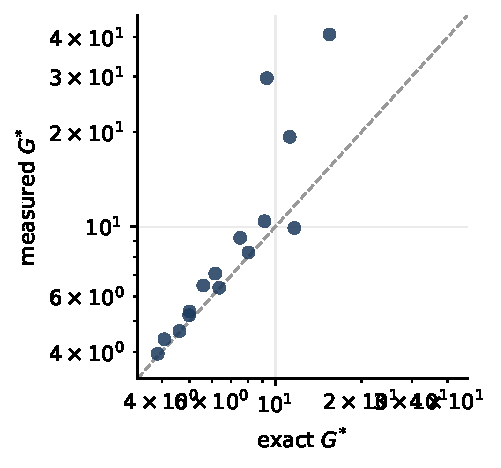
\includegraphics[width=0.92\linewidth]{figures/estimator_accuracy.pdf}
  \caption{Measured against exact optimal group size across prompt pools.}
  \label{fig:estimator-accuracy}
\end{figure}

\subsection{Transformers trained from scratch}

A population of independent transformers is warmed up on a verifiable running-sum task until each
member reaches a common pass rate, the noise terms are measured at that frozen policy, and every
member is then trained from the same starting point at each split of a fixed rollout budget. The
corpus size is the knob: sampling without replacement from a corpus of $N$ scales the between-prompt
term by $1 - (P-1)/(N-1)$, so shrinking the corpus toward the batch raises $G^{\star}$ without touching
the task.

\begin{table*}[t]
  \centering
  \begin{tabular}{lcccccc}
\toprule
corpus $N$ & $\tau_b$ & $\tau_w$ & predicted $G^{\star}$ & best measured $G$ & Spearman & $R^2$ \\
\midrule
128 & 32.1 & 137.1 & 3.06 & 2 & +0.943 & 0.983 \\
192 & 35.4 & 140.3 & 2.98 & 2 & +0.943 & 0.954 \\
512 & 37.6 & 146.8 & 2.97 & 2 & +0.943 & 0.987 \\
4096 & 37.7 & 141.8 & 2.94 & 4 & +1.000 & 0.984 \\
unbounded & 37.3 & 140.0 & 2.94 & 4 & +1.000 & 0.985 \\
\bottomrule
\end{tabular}
  \caption{Predicted and measured optimum on transformers trained from scratch. The sweep visits
  $G \in \{2, 4, 8, 16, 32, 64\}$, so a predicted optimum near three can only appear as a peak at
  two or four; those two are within one standard error of each other in four of the five corpora,
  and every corpus shows the predicted decline beyond $G = 8$. Spearman and $R^2$ are computed
  against the parameter-free prediction across the whole sweep.}
  \label{tab:transformer}
\end{table*}

\begin{figure*}[t]
  \centering
  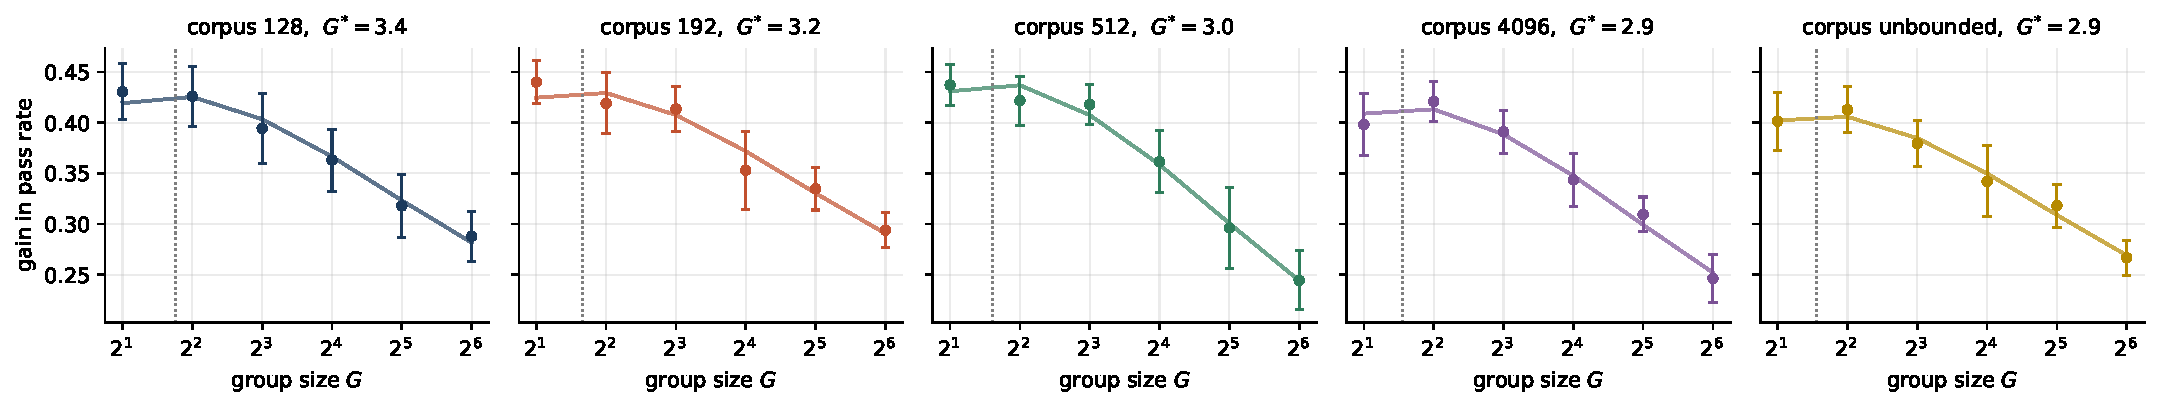
\includegraphics[width=\textwidth]{figures/transformer_curves.pdf}
  \caption{Gain against group size at a fixed rollout budget, with the parameter-free prediction
  overlaid and the predicted $G^{\star}$ marked.}
  \label{fig:transformer-curves}
\end{figure*}

\subsection{Under Adam}
\label{sec:adam}

Everything above is under plain gradient ascent, where the update is the gradient and the noise can
be read in the parameter metric. Real runs use Adam, which moves in a different metric and is scale
invariant, so the theory only carries over if the noise is measured after preconditioning. Repeating
the sweep under both optimisers gives Table~\ref{tab:adam}.

\begin{table*}[t]
  \centering
  \begin{tabular}{lcccccccc}
\toprule
gain by group size & 2 & 4 & 8 & 16 & 32 & 64 & measured $G^{\\star}$ & $R^2$ \\
\midrule
gradient ascent & +0.409 & +0.413 & +0.390 & +0.333 & +0.300 & +0.250 & 2.94 & 0.992 \\
Adam & +0.519 & +0.527 & +0.514 & +0.492 & +0.447 & +0.384 & 3.42 & 0.969 \\
\bottomrule
\end{tabular}
  \caption{The same sweep under gradient ascent and under Adam. The optimum is at $G = 4$ for both,
  and the predicted curve explains the measured one about as well. The measured $G^{\star}$ for Adam is
  taken in Adam's own metric, which takes some care -- see below.}
  \label{tab:adam}
\end{table*}

The law survives, but measuring in Adam's metric required fixing two things, and both are
consequences of the preconditioner being an estimated quantity rather than a fixed one.

First, a probe run at a frozen policy starts with an empty second-moment estimate, so there is no
metric to measure in yet. Priming it -- running the optimiser's state forward on real batches with
a zero step size, so the policy does not move -- gives the preconditioner a real run would have.

Second, and less obviously, dividing by $\sqrt{v}$ is unbounded. Coordinates that rarely receive
gradient have a tiny second moment, which is harmless for the update, since Adam's update is
bounded by construction, but ruinous for an inner product between two noisy gradients: those
coordinates dominate it. Measured this way the estimator returned $\tau_b < 0$ and an inverted
efficiency curve. Flooring the second moment at a fraction of its own mean before dividing fixes
it, and the result is insensitive to where the floor is put: over three orders of magnitude in the
floor, the measured $G^{\star}$ moves only from $3.51$ to $3.15$, against an observed optimum of $4$.
Without a floor the same measurement reports $11.9$.

This is the one place where our quantities need care that the plain-gradient case does not. The
working rule is to instrument the update rather than the gradient, and to floor the preconditioner
before inverting it.

\subsection{A pretrained model}

We repeat the measurement on Qwen2.5-0.5B-Instruct with LoRA adapters as the trainable parameters,
over corpora of short exact-match tasks: counting a letter in a word, naming the $k$-th item of a
list, adding two numbers, and a mixture of all of them. Measured optimal group sizes run from $2.7$
to $6.2$, the same range as the enumerable policies and the transformers trained from scratch.

Corollary~\ref{cor:bernoulli} predicts that the within-prompt noise tracks the reward histogram at a
fixed score scale, and difficulty buckets inside one family are where that assumption is tenable.
We screen prompts with a larger sample than the measurement uses, so the bucket boundaries do not
inherit the noise of the quantity under test, and report the pass rate re-measured during the probe
rather than the one used to sort. Across buckets spanning pass rates from $0.25$ to $0.30$, the
ratio $\tau_w/\E[p(1-p)]$ is constant to within $14\%$ (Table~\ref{tab:difficulty}).

\begin{table*}[t]
  \centering
  \small
  \emph{pending: this table is generated from a run that has not been stored yet.}
  \caption{Within-prompt noise across difficulty buckets of one task family. The gap between the
  screened and re-measured pass rates in the outer buckets is regression to the mean, which is why
  the screening sample is the larger of the two.}
  \label{tab:difficulty}
\end{table*}

Across \emph{different} families the same ratio varies by a factor of $8.8$
(Appendix~\ref{app:cross-family}), and the reason is visible in the assumption: the constant the corollary
predicts is the score scale $\sigma_s^2$, and a family whose answer is one number does not share a
score scale with one whose answer is four. This bounds how the corollary should be used. It
converts a reward histogram into a noise estimate within a task distribution, after one calibration
measurement, and it does not transport that calibration to a task of a different shape.

\subsection{What the hardware is worth}
\label{sec:hardware}

Theorem~\ref{thm:split} turns the split into a question about the serving stack as much as about
the learning problem, through the prefill ratio $\alpha = c_{\mathrm{pre}}/c_{\mathrm{dec}}$. We
measured both costs for a $0.5$B model in bfloat16 on the machine everything else ran on. The ratio
is governed almost entirely by the prompt-to-response length ratio, running from $0.04$ when a
short prompt is followed by a thousand tokens of response to $10.9$ when a thousand-token prompt is
followed by a short answer.

\begin{table*}[t]
  \centering
  \small
  \begin{tabular}{lcccc}
\toprule
$c_{\mathrm{pre}}/c_{\mathrm{dec}}$ & $R=64$ & $R=256$ & $R=1024$ & $R=8192$ \\
\midrule
0.00 & 2.9 & 2.9 & 2.9 & 2.9 \\
0.04 & 3.0 & 3.0 & 3.1 & 4.0 \\
0.70 & 3.6 & 4.0 & 5.5 & 13.1 \\
2.63 & 5.0 & 6.2 & 9.7 & 25.1 \\
10.92 & 8.7 & 11.5 & 19.2 & 51.0 \\
\midrule
\multicolumn{5}{l}{\footnotesize small-batch limit \eqref{eq:gstar-cost} --- $\alpha=0.00$: 2.9, $\alpha=0.04$: 2.9, $\alpha=0.70$: 3.5, $\alpha=2.63$: 4.6, $\alpha=10.92$: 7.6} \\
\bottomrule
\end{tabular}
  \caption{The optimum $G^{\star}$ from Theorem~\ref{thm:split}, at the noise ratio measured on our
  transformers, across measured prefill ratios and rollout budgets. Entries are the root of
  \eqref{eq:stationary}, which agrees with direct numerical minimisation of \eqref{eq:objective} to
  one part in $10^{7}$. The last row shows the small-batch limit, which is what one would quote
  from \eqref{eq:gstar-cost} alone and which understates the optimum badly at large $R$.}
  \label{tab:optimum}
\end{table*}

\begin{figure}[t]
  \centering
  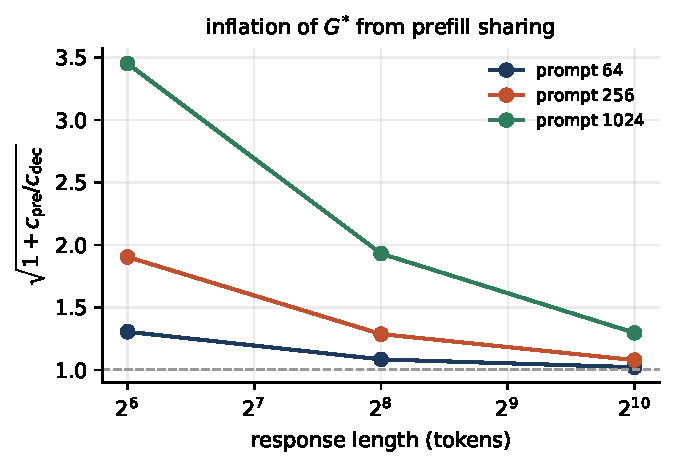
\includegraphics[width=\linewidth]{figures/cost_model.pdf}
  \caption{Measured prefill-to-decode economics on an Apple M4, as the group-size inflation implied
  in the small-batch limit. Long responses make prefill sharing almost worthless; short answers
  behind long prompts make it decisive.}
  \label{fig:cost-model}
\end{figure}

Table~\ref{tab:optimum} is the reconciliation the paper has been building towards. A purely
statistical reading of the split says three; the settings in which published recipes were developed
say otherwise, and the theorem says how much of that is justified. Long prompts with short answers
at a large batch put the optimum in the tens, which is where the recipes are. Reasoning-length
responses, where the response dwarfs the prompt, put it back at three to four, and there a group of
sixteen is spending most of its budget on responses that a second prompt would have used better.
The disagreement between a recipe and this analysis is therefore not evidence against either: it
identifies the regime the recipe came from.

\subsection{What transfers when the batch size changes}

The sharpest consequence of the drift model is a statement about transfer. A run tuned by learning
rate is tuned in a unit that depends on the batch through $\mathcal{G} + N/P$; a run tuned by drift
is not. Table~\ref{tab:transfer} sweeps both parameterisations at four batch sizes and reports what
it costs to carry the value tuned at the smallest batch to the others.

\begin{table*}[t]
  \centering
  \begin{tabular}{lcccc}
\toprule
prompts per step $P$ & 8 & 16 & 32 & 64 \\
\midrule
best step size $\eta^{*}$ & 0.0417 & 0.0786 & 0.1228 & 0.1615 \\
best drift target $D^{*}$ & 5.06e-03 & 5.29e-03 & 5.15e-03 & 3.98e-03 \\
cost of transferring $\eta$ (\%) & +0.0 & -9.9 & -17.9 & -22.0 \\
cost of transferring $D^{*}$ (\%) & +0.0 & +0.0 & +0.0 & +0.0 \\
\bottomrule
\end{tabular}
  \caption{Transfer across batch size. The learning rate that is optimal at $P = 8$ loses a fifth of
  the achievable gain by $P = 64$; the drift target that is optimal at $P = 8$ remains optimal.}
  \label{tab:transfer}
\end{table*}

\begin{figure*}[t]
  \centering
  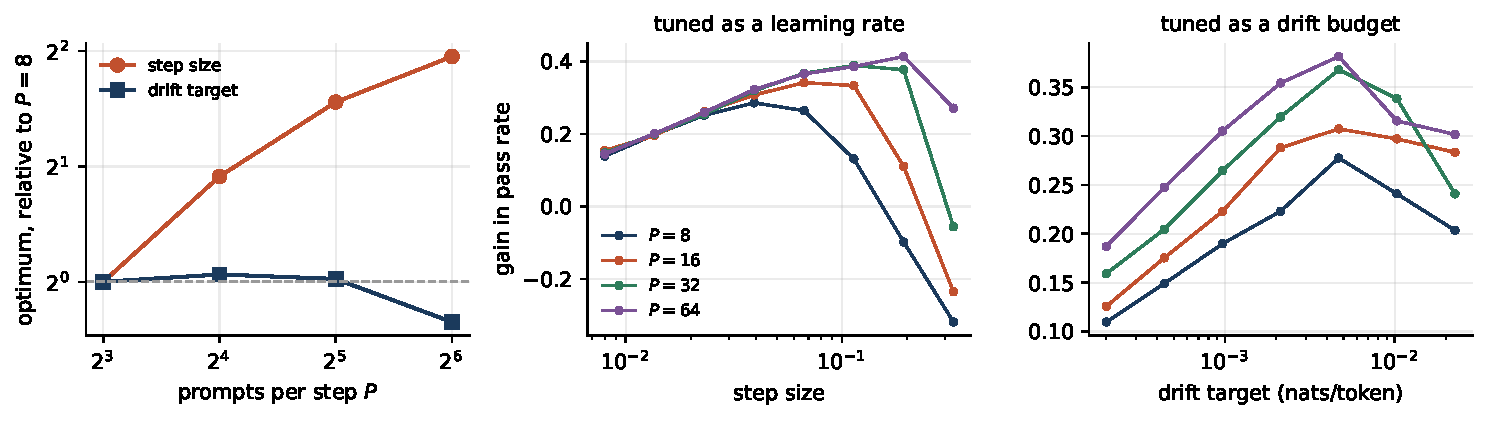
\includegraphics[width=\textwidth]{figures/transfer.pdf}
  \caption{Left: the optimum of each parameterisation relative to its value at $P = 8$. Centre and
  right: the sweeps themselves. The learning-rate optimum moves; the drift optimum does not.}
  \label{fig:transfer}
\end{figure*}

The single-step drift model accounts for part of the movement in $\eta^{*}$ and not all of it: the
coefficient $\mathcal{G} + N/P$ measured at the initial policy predicts a smaller shift than the one
observed over a full run. The coefficient keeps moving as the policy improves, so a controller that re-reads it tracks the
optimum while a learning rate fixed in advance cannot.

\subsection{A prospective test, and where the drift target stops transferring}
\label{sec:recipe}

Everything so far tunes one quantity at a time on the setting it is measured on. The stronger test
is prospective: fix a setting the method has never seen, let the probe choose $G$ before any
training happens, and check afterwards whether it chose well. We moved to a held-out setting with
four times the rollout budget, eight times the corpus and a different seed. The probe reported
$G^{\star} = 3.1$, so the recipe took $G = 4$; the comparison is against $G = 16$, which is what a
default recipe would use.

\begin{table}[t]
  \centering
  \small
  \begin{tabular}{lcc}
\toprule
best achievable gain & $G = 4$ & $G = 16$ \\
\midrule
tuning a learning rate & +0.4947$^{\ast}$ & +0.4780$^{\ast}$ \\
tuning a drift target & +0.4431 & +0.3989 \\
predicted efficiency $\rho$ & 0.815 & 0.674 \\
\bottomrule
\end{tabular}
  \caption{Best achievable gain at the held-out setting, crossing the group size the probe selected
  against the group size a default recipe would use, under both ways of setting the step. Starred
  entries sit at the edge of their grid and are lower bounds. The probe's choice wins under both.}
  \label{tab:diagnosis}
\end{table}

\textbf{The prospective choice was right.} $G = 4$ beats $G = 16$ under both parameterisations.
Under drift control, where the step size is held to the same behavioural budget in both arms and so
cannot confound the comparison, it wins by $11.1\%$ against a predicted
$\sqrt{\rho_4/\rho_{16}} - 1 = 10\%$.

\textbf{The drift target transfers across the group size exactly.} Both group sizes put their
optimum at the same drift target, $1.45 \times 10^{-3}$. Changing how the budget is split does not
change how far the policy should move per update, which is what a behavioural unit ought to do.

\textbf{It does not transfer across this change of budget.} The tuning setting's optimum was
$3.19 \times 10^{-3}$, a factor of $2.2$ away, and carrying it over costs $20\%$ of the achievable
gain. Earlier the same target held to within $5\%$ across a fourfold change in batch size and
$21\%$ across an eightfold one. A sixteenfold change in prompts per step, combined with a fourfold
change in rollout budget, is past where a single number holds. We found this the hard way: packaging
the two together and carrying both to the held-out setting lost to the default by $28.9\%$ (paired
$t = -3.01$ over $32$ runs), and Table~\ref{tab:diagnosis} is what attributes that loss to the drift
target rather than to the group size.

\textbf{A constant drift target is not the right schedule.} At both group sizes a tuned constant
learning rate beat the best constant drift, with its optimum at the edge of the grid. A fixed
learning rate produces a drift that changes over a run as the gradient statistics change, and that
this wins says the optimal drift trajectory is not flat. The unit appears to be right and the
schedule is not, which is the most concrete thing this paper leaves open.

\section{Related work}
\label{sec:related}

\paragraph{Batch size and gradient noise.} The gradient noise scale predicts the batch size beyond
which data parallelism stops buying speed, and does so from statistics measurable during training
\citep{mccandlish2018empirical}; the empirical picture across tasks and optimisers is mapped in
\citet{shallue2019measuring}. Both concern a single level of sampling. RLVR samples prompts and then
samples responses within each prompt, and the resulting two-level noise scale, the split it implies,
and the fact that the response-level term is readable off the reward histogram, have no counterpart
in that literature. The variance decomposition itself is the classical two-stage sampling result
\citep{cochran1977sampling}, applied here to policy gradients.

\paragraph{Hyperparameter transfer.} $\mu$P makes learning rates transfer across width by fixing what
a step does to the network's functions rather than to its parameters
\citep{yang2021tensor, yang2022mutransfer}. This paper takes the same stance one level up: fix what
a step does to the policy's \emph{behaviour}, measured as drift in nats per token, and the recipe
transfers across batch size. We find no comparable prescription for RL post-training in the
literature; the closest work reports empirical scaling behaviour and fitted power laws
\citep{tan2025scalingbehaviors, khatri2025artofscaling, ghosh2026predictable} rather than a
quantity to hold fixed.

\paragraph{Estimators for RLVR.} RLOO \citep{ahmadian2024rloo, williams1992reinforce}, GRPO
\citep{shao2024deepseekmath}, its unnormalised correction \citep{liu2025drgrpo}, DAPO
\citep{yu2025dapo} and sequence-level variants \citep{zheng2025gspo} are usually compared by
benchmark deltas. Proposition~\ref{prop:mean} shows that, for binary rewards, the members of this
family differ only through a difficulty weight $\lambda(p, G)$, that a $p$-independent $\lambda$ is
absorbed exactly by the step size, and that standardisation is a change of objective rather than a
variance reduction -- a sharpening of the argument in \citet{liu2025drgrpo}. Recent analyses of why
normalisation helps \citep{ge2026normalization} and of what outcome-reward objectives cannot
simultaneously be \citep{ding2026impossibility} are complementary: they characterise the estimator,
while the question here is how many samples to give it and how far to step.

\paragraph{Allocating rollouts.} Several recent methods vary the number of responses per prompt
within a batch using heuristics tied to observed pass rates or gradient variance
\citep{nguyen2026allocation}, or adapt the batch size from a divergence signal
\citep{park2026batchscaling}, and one line of work argues for scaling the response count
specifically \citep{hu2025brorl}. These are allocation policies; what has been missing is the
quantity being optimised. Equation~\eqref{eq:gstar} supplies it in closed form and shows that the
answer is a ratio of two measurable traces, which also explains why heuristics keyed to pass rate
alone succeed on some corpora and not others: pass rate determines $\tau_w$ but says nothing about
$\tau_b$.

\paragraph{Trust regions and KL control.} Constraining how far a policy moves is old
\citep{schulman2015trpo, schulman2017ppo} and its modern LLM forms clip importance ratios or
penalise divergence from a reference. The drift used here is neither: it is the KL between
\emph{consecutive} policies, used as a measurement and a control target rather than as a penalty,
and its role in this paper is to supply the unit in which a recipe transfers.

\paragraph{Asynchrony and off-policy correction.} A parallel literature studies what happens when
the sampling policy and the training policy differ, whether through pipeline staleness
\citep{song2026staleness} or numerical mismatch between rollout and training engines. That work
asks how much mismatch a run tolerates. This paper asks a question that arises before any mismatch:
given that the sampler and the trainer agree, how should the sampling budget be divided, and how
large a step should the result support.

\section{Discussion}
\label{sec:discussion}

\paragraph{What a practitioner should take from this.} Three things, in decreasing order of how
confident we are in them. Running longer does not cost reproducibility: the spread across seeds is
flat in the number of updates, so there is no reason to cut a run short to keep results stable.
Batch composition is the dominant lever, and it acts as $P^{-1/2}$, so the returns are real but slow
-- quadrupling the batch halves the spread. And the step size matters less than one would expect,
entering as $D^{+1/2}$, which means a run can be made faster without being made much less
reproducible, up to the saturation boundary below.

\paragraph{On reporting.} The honest consequence of Section~\ref{sec:exp-seeds} is not that error
bars are now free. It is that they are cheap in a way they were not: the scaling transfers, so one
calibration -- a handful of seeds at one setting -- lets a practitioner carry an error bar across
changes of batch and step size, which is where most of the variation between reported configurations
comes from. What we could not deliver is the absolute level from a single run, and
Section~\ref{sec:exp-seeds} says exactly why the obvious route fails.

\paragraph{Against drift targeting, in one case.} Section~\ref{sec:drift} recommends specifying a
run by a drift target rather than a learning rate, and Section~\ref{sec:experiments} shows that
target transferring across batch size where a learning rate does not. Section~\ref{sec:exp-seeds}
shows the same technique destroying two runs. The mechanism is specific and worth stating plainly:
$\E_x[p(1-p)] \to 0$ as a task is solved, the signal goes with it, and a controller holding drift
constant answers by raising the step without bound. Any drift-targeted schedule needs a floor on the
signal or a cap on the step; ours had neither.

\paragraph{Limits.} The linearisation behind Proposition~\ref{prop:stationary} assumes the two runs
stay close enough that the mean gradient field is locally linear between them, which is the same
assumption that fails at saturation. The largest model measured is $0.5$B parameters, and the tasks
are short-answer and exactly verifiable; whether the same picture holds for reasoning-length
responses, where a single rollout carries far more entropy, is the obvious next measurement and we
have not made it. The contraction time is treated as a single number and is not one. And the
estimator family of \eqref{eq:family} excludes clipping, which makes the update a nonlinear function
of the batch and breaks the linearity the noise decomposition relies on.

\paragraph{What we would do next.} Measure the spectrum of the contraction rather than a single
timescale, since that is what stands between the scaling law and an absolute error bar. Repeat the
measurement where responses are long, which is both the regime that matters most and the one where
the within-prompt noise term should be largest. And check whether the same balance explains a
phenomenon we did not set out to study: if divergence between two seeds is stationary, then so is
divergence from any perturbation, including a change of data order or of hardware numerics, and the
same instrument should predict those.


\bibliography{refs}

\appendix
\section{Proofs of the exact moment results}
\label{app:proofs}

\subsection*{Proposition~\ref{prop:mean}}
\begin{proof}
  Condition on $r_j$. The other $G-1$ rewards are i.i.d.\ Bernoulli$(p)$ and, given $r_j$, are
  independent of $\score(y_j)$, so
  $\E[w(k, r_j)\score(y_j)] = \sum_{r} \Pr[r]\, W_r\, u_r$. Summing over $j$ and applying
  \eqref{eq:score-identity} gives $\E[z] = p\,(W_1 - W_0)\,u_1 = \lambda h$.
\end{proof}

\subsection*{Proposition~\ref{prop:cov}}
\begin{proof}
  Split $\E[z z^{\!\top}]$ into diagonal and off-diagonal terms. The diagonal contributes
  $G^{-1}[p Q_1 M_1 + (1-p) Q_0 M_0]$ with $M_r = S_r + u_r u_r^{\!\top}$. For $j \neq l$,
  condition on $(r_j, r_l)$ and on the count $m'$ among the remaining $G-2$ responses; the two
  scores are then conditionally independent, giving
  $\frac{G-1}{G}\sum_{a,b}\Pr[a]\Pr[b]\,C_{ab}\,u_a u_b^{\!\top}$, which collapses to
  $\frac{G-1}{G} p^2 (C_{11} - 2C_{10} + C_{00}) U$ by \eqref{eq:score-identity}. Subtracting
  $\E[z]\E[z]^{\!\top} = \lambda^2 p^2 U$ completes the proof.
\end{proof}

\section{Reproducing the results}
\label{app:repro}

Every figure and table is regenerated from stored run records by
\texttt{analysis/figures.py} and \texttt{analysis/tables.py}, and so is every headline number in
the prose: they are emitted as macros into \texttt{tables/numbers.tex} and referenced rather than
typed, so a rerun that moves a number moves it in the text as well. Each run writes a manifest holding the configuration, its hash, the commit the
code was at, and the interpreter and platform it ran on.

The exactness tests in \texttt{tests/} check every analytic result in Section~\ref{sec:theory}
against brute-force enumeration, and check the batched estimator against the reference
implementation term by term. Theorem~\ref{thm:adjoint} is additionally checked against the same
quantity assembled the expensive way, by building $S_T$ explicitly and forming
$\nabla M^{\!\top} S_T \nabla M$, and Proposition~\ref{prop:potential} against the measured
asymmetry of $\mathcal{J}$, which is $3\times10^{-10}$ across the estimator family, at the finite-difference
floor.

\paragraph{Evaluation randomness, and a bracket instead of a rerun.} Recovering a seed term from
the spread of an estimated score means subtracting the evaluation's own binomial variance, and that
subtraction assumes each run drew its own evaluation. The seven-billion runs were scored before we
noticed this, sharing one draw. Re-scoring them costs hours at that size, and is unnecessary: shared
evaluation noise is common to every run and so drops out of the variance between them, while
independent noise adds to it, which brackets the seed term between the observed spread and the
binomially corrected one whatever was actually shared. At $7$B those two ends differ by $0.3\%$,
because the binomial term is small against a spread that large. The smaller model was re-run with
independent draws, where the correction matters more.

\paragraph{One thing that was not reproducible, and now is.} The LoRA adapters are attached by
\texttt{mlx\_lm}, which draws their $A$ matrices from a generator that is not seeded by default.
Every process therefore began from a different parameterisation. The policy was the same either way,
because the $B$ matrices start at zero, and every seed within a run shares one initialisation, so
the spreads reported here are unaffected: the runs being compared differ only in rollout randomness,
as claimed. What was affected is repetition. Rerunning the same configuration gave different
numbers, which we noticed when a rerun of one experiment disagreed with itself. The initialisation
is now seeded from the run's configuration, and the released tests check that two attachments at one
seed agree and that two seeds do not.

\paragraph{What each thing costs.} Everything here ran on one Apple M4 laptop with $24$\,GB of
unified memory, and the costs are worth stating because they bound what a reader can repeat. The
enumerable-policy experiments are CPU work and finish in minutes; the $\numForecastSettings$-setting
forecast grid, which trains $\numForecastSeeds$ runs in each of them, takes about half an hour. The
populations of small transformers take a few hours each. On the pretrained models the arithmetic
changes: a single Qwen2.5-0.5B run of twelve updates takes about three minutes and its backward
pass about ten, while one Qwen2.5-7B run of twenty updates takes around an hour, so the eight-seed
measurement at $7$B is most of a day. That last figure is the reason this paper stops where it
does.

\paragraph{Using the backward pass elsewhere.} Algorithm~\ref{alg:forecast} needs two things from
a training run and nothing else: the variance across prompts of the batch gradient projected onto a
direction, and a Jacobian-vector product of the mean update field with that direction. The released
code states that as a protocol rather than a class hierarchy, so a trainer in another framework
implements two methods and reuses the recursion. Two implementations ship with it, one for
enumerable policies where every term is exact and one for a pretrained model through MLX. Both are
tested against systems whose answer is available in closed form: the protocol against linear
Gaussian recursions, and the pretrained-model implementation against a stand-in with the same
interface whose mean update field is a fixed linear map, which exercises the finite-difference
Hessian-vector product without needing a model to run it on.

One numerical detail is worth recording. The difference step $\epsilon$ has a floor set by the
precision the weights are held in: below roughly $10^{-4}$ in float32 the two evaluations cancel
into rounding error rather than into a derivative. We use $10^{-3}$, which sits above that floor and
well below the scale on which the gradient field bends.

\paragraph{A claim index.} The released code carries \texttt{docs/claims.md}, which lists every
claim in this paper against the experiment that produced it and how strongly it is supported:
exact, measured with an interval, observed without one, or a negative result. It also lists what we
withdrew and what we do not claim. It is written for a reader who distrusts one particular number
and wants to find its source without reading the code.

\paragraph{Which experiment produces what.}
\begin{itemize}\itemsep1pt
  \item \texttt{p1\_propagation}: the covariance recursion against Monte Carlo
    (Table~\ref{tab:propagation}, Figure~\ref{fig:teaser} right).
  \item \texttt{p2\_metric\_forecast}: the prospective forecast
    (Table~\ref{tab:forecast}, Figures~\ref{fig:teaser} left and \ref{fig:forecast}).
  \item \texttt{p3\_memory\_sources}: attribution and the memory horizon
    (Figure~\ref{fig:sources}, Section~\ref{sec:exp-forecast}).
  \item \texttt{p4\_linearity}: the linearisation residual (Section~\ref{sec:exp-linearity}).
  \item \texttt{p5\_adam\_lift}: the lifted recursion (Table~\ref{tab:adam-lift}).
  \item \texttt{p6\_spectrum}: the spectrum of the transfer operator (Table~\ref{tab:spectrum}).
  \item \texttt{s1}, \texttt{s3}, \texttt{s5}: seed divergence on transformers and on a pretrained
    model (Figures~\ref{fig:reconvergence} and \ref{fig:real-seeds}).
  \item \texttt{s6\_scale}: the seven-billion-parameter measurements
    (Section~\ref{sec:exp-scale}).
  \item \texttt{s7\_real\_forecast}: the backward pass on a pretrained model, and
    \texttt{power.py} the simulation of what that design can resolve
    (Appendix~\ref{app:power}).
  \item \texttt{s8\_null}: the same run with the reward replaced by a coin
    (Table~\ref{tab:signal}, Figure~\ref{fig:null}).
  \item \texttt{a}, \texttt{b}, \texttt{c}, \texttt{d}, \texttt{t}: the estimator, allocation and
    cost-model results of Section~\ref{sec:applications}.
\end{itemize}

The exact-tier experiments run in minutes on a laptop CPU. The pretrained-model experiments need
Apple Silicon and MLX; the seven-billion-parameter runs need about $24$\,GB of unified memory, and
the eight-seed sweep takes several hours.

\section{What the real-model design can resolve}
\label{app:power}

The seed spread of a score estimated from a finite evaluation is recovered by subtracting the
evaluation's own binomial variance from the observed spread across runs. That is a difference of
two noisy quantities, and below some true spread it is not distinguishable from zero. Reporting a
number from it without knowing where that boundary lies would be reporting noise.

\begin{table}[t]
  \centering
  \footnotesize
\setlength{\tabcolsep}{4pt}
\begin{tabular}{@{}lcccc@{}}
\toprule
& \multicolumn{2}{c}{6 runs} & \multicolumn{2}{c}{8 runs} \\
\cmidrule(lr){2-3} \cmidrule(lr){4-5}
true s.d. & resolved & estimate & resolved & estimate \\
\midrule
0.000 & 50\% & 0.000 & 46\% & 0.000 \\
0.010 & 58\% & 0.007 & 72\% & 0.009 \\
0.020 & 83\% & 0.018 & 88\% & 0.018 \\
0.040 & 99\% & 0.034 & 99\% & 0.039 \\
0.080 & 100\% & 0.069 & 100\% & 0.076 \\
\bottomrule
\end{tabular}
  \caption{Simulating the design as run, with $48$ held-out questions and $16$ samples each at a
  pass rate near $0.35$, over a range of true seed spreads. \emph{Resolved} is the fraction of trials in
  which the subtraction returns something positive; \emph{estimate} is the median of what it
  returns.}
  \label{tab:power}
\end{table}

Three readings from Table~\ref{tab:power}, and the first is a warning about the method rather than
about the data. At a true
spread of zero the subtraction still returns a positive number in about half of trials, because a
difference of two noisy variances is positive half the time. A non-zero reading is therefore not by
itself evidence of a seed spread; the interval is.

Second, the design resolves what it needs to. At a true spread of $0.02$ the subtraction recovers
something in $88\%$ of trials at eight runs and lands at a median of $0.018$; at $0.04$ it succeeds
essentially always. Those bracket the forecast we make.

Third, the bootstrap interval is anti-conservative here: its coverage of the true value runs from
$68\%$ to $88\%$ rather than the nominal $95\%$, which is the percentile bootstrap applied to a
variance difference at small $n$. We report the intervals because they are far more informative
than a point estimate, and note that they are narrower than they should be.

\section{The estimator family as a table}
\label{app:family}

Because the advantage depends only on $(k, r)$, an estimator is a $(G+1) \times 2$ array, and the
moments in \eqref{eq:contractions} are contractions of that array against a binomial distribution.
This is what makes the exact treatment cheap: no sampling is involved in evaluating
$\lambda(p, G)$, $Q_r$ or $C_{ab}$ for any member of the family, at any group size.


\section{Noise terms across task families}
\label{app:cross-family}

The corollary relating within-prompt noise to the reward histogram assumes a shared score
scale, which holds within a task family and not between families of different answer shape.
Table~\ref{tab:real} and Figure~\ref{fig:real-model} make the size of that effect explicit.

\begin{table*}[t]
  \centering
  \small
  \begin{tabular}{lcccccc}
\toprule
corpus & pass rate & $\E[p(1-p)]$ & $\tau_b$ & $\tau_w$ & $G^{*}$ & $\tau_w/\E[p(1-p)]$ \\
\midrule
count letter & 0.280 & 0.178 & 4.35e+02 & 1.16e+04 & 6.15 & 0.27 \\
nth word & 0.326 & 0.138 & 4.88e+03 & 2.01e+04 & 3.03 & 0.61 \\
add two & 0.546 & 0.062 & 1.29e+04 & 3.55e+04 & 2.66 & 2.40 \\
mixed & 0.193 & 0.071 & 4.31e+03 & 1.20e+04 & 2.67 & 0.71 \\
\bottomrule
\end{tabular}
  \caption{Noise terms measured on a pretrained model. The last column would be constant if the
  score scale were shared across families; it is not, and it is not meant to be.}
  \label{tab:real}
\end{table*}

\begin{figure}[t]
  \centering
  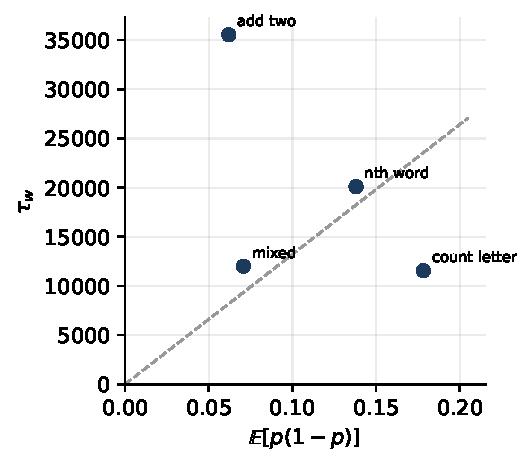
\includegraphics[width=0.95\linewidth]{figures/real_model.pdf}
  \caption{Within-prompt noise against the reward histogram across corpora, with a single fitted
  scale. The scatter is the score scale differing between task families.}
  \label{fig:real-model}
\end{figure}


\end{document}
